% Asset ID: A21FunctionsAndGraphsTIKZ-008
% Unit: A21: A2 1 Pure Mathematics
% Topic code: A21-AF
% Related LO IDs: A21-AF-LO006, A21-AF-LO007
% Related lesson section: Solving a Transformed Modulus Problem
% Source: Chapter 2 Functions and Graphs transformed modulus section
% Purpose: Show the graph of y = 3|x - 1| - 2 and its intersections with y = 1/2 x + 3.

\documentclass[tikz,border=8pt]{standalone}
\usepackage{amsmath}
\usetikzlibrary{arrows.meta}
\begin{document}
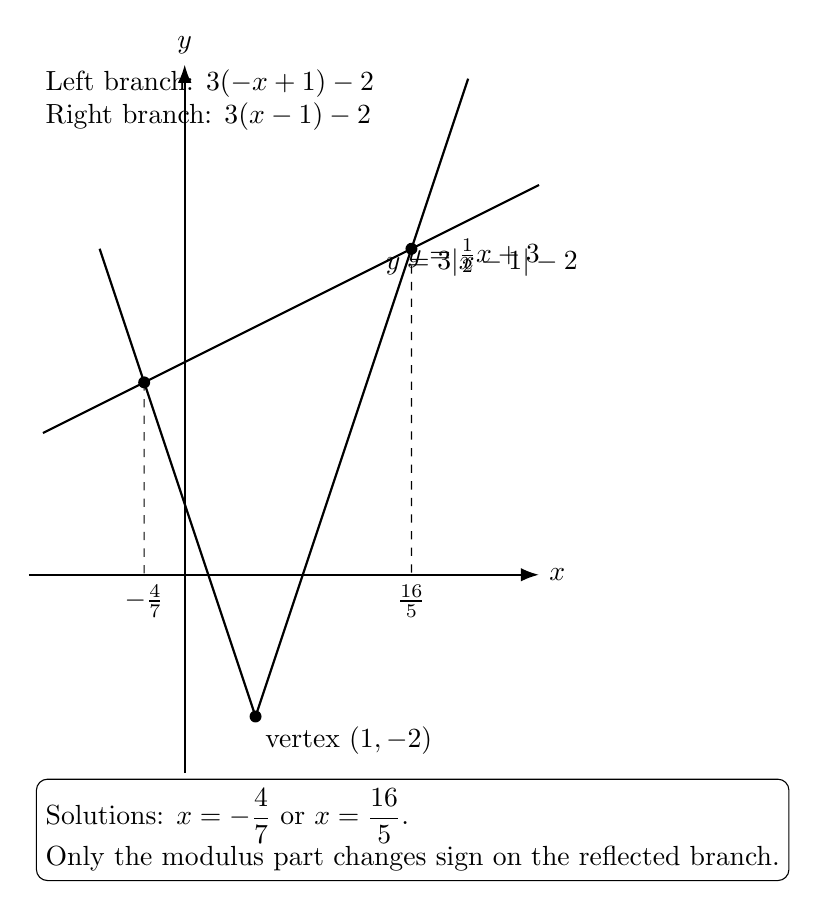
\begin{tikzpicture}[scale=0.9, >=Latex]
\draw[->, thick] (-2.2,0) -- (5,0) node[right] {$x$};
\draw[->, thick] (0,-2.8) -- (0,7.2) node[above] {$y$};
\draw[thick] (-1.2,4.6) -- (1,-2) -- (4,7);\node[right] at (2.7,4.4) {$y=3|x-1|-2$};
\draw[thick] (-2,2) -- (5,5.5);\node[right] at (3,4.5) {$y=\frac12x+3$};
\coordinate (A) at (-0.5714,2.7143);\coordinate (B) at (3.2,4.6);
\fill (A) circle (2.4pt);\fill (B) circle (2.4pt);
\draw[dashed] (A) -- (-0.5714,0);\draw[dashed] (B) -- (3.2,0);
\node[below] at (-0.5714,0) {$-\frac47$};\node[below] at (3.2,0) {$\frac{16}{5}$};
\fill (1,-2) circle (2.4pt);\node[below right] at (1,-2) {vertex $(1,-2)$};
\node[align=left, anchor=west] at (-2.1,6.7) {Left branch: $3(-x+1)-2$\\Right branch: $3(x-1)-2$};
\node[draw, rounded corners, align=left, anchor=west] at (-2.1,-3.6) {Solutions: $\displaystyle x=-\frac47$ or $\displaystyle x=\frac{16}{5}$.\\Only the modulus part changes sign on the reflected branch.};
\end{tikzpicture}
\end{document}
